\section{Experiment and Discussion}
\subsection{Evaluation for Co-segmentation on Synthetic Data}
\begin{figure}[htb]
	\centering
	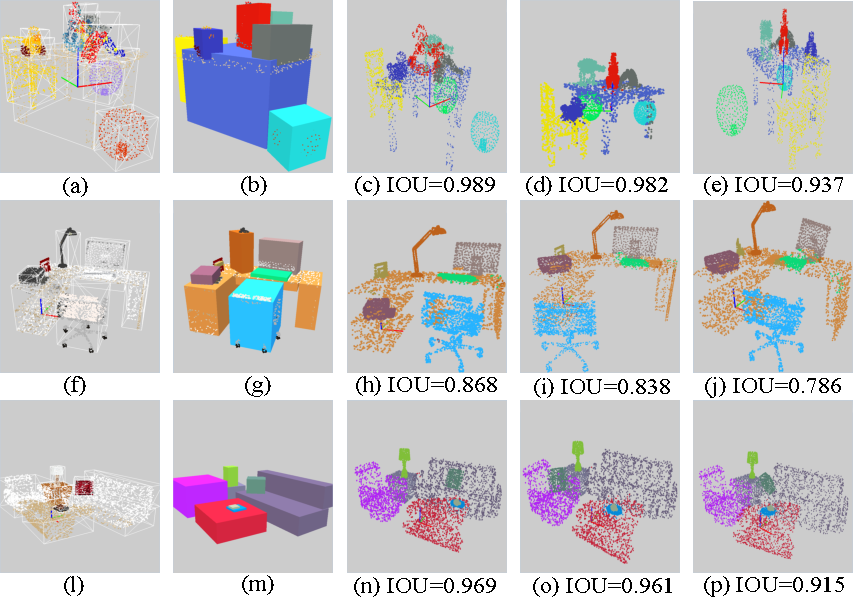
\includegraphics[width=\linewidth]{images/seg/seg}
	\caption{\label{fig:seg}Three rows in the figure shows segmentation evaluations on three groups of synthetic data (child table, office desk, living room). Each group of data have 13 point sets. The first column are examples of point sets for each group of data. The second column are mannual placed layout for each group of data. The $3^{rd}$ column shows the segmentation result with maximum IOU scores in the groups. The $4^{th}$ column shows the segmentation result with median IOU scores in the groups. The $5^{th}$ column shows the segmentation result with minimum IOU scores in the groups.}
\end{figure}
From the perspective of co-segmentation, we evaluate our algorithm on synthetic data of indoor scenes. To estimate the power of the algorithm we only input layout for one point set in each group for initialization and do not use the hot intervention mechanism. For numercial estimation, we calculate the intersection over union (IOU) scores for the result segmentation against ground-truth segmentation. We generate three group of synthetic point sets and each group have 13 point sets as inputs. The Figure~\ref{fig:seg} shows the result of the evalution.\\
From the evaluation, we want to discuss one interesting observation:\\
For all three groups, the point set with highest IOU score is not the same as the point set equiped with mannually placed layout.In other words , the point sets from the $3^{rd}$ column in Figure~\ref{fig:seg} are not the same point sets from $2^{nd}$. In the first group of data (dataset of child table in Figure~\ref{fig:seg}), the segmentation result of the point set with layout is even the second worst in the sense of IOU score. We believe this is because that the mannually placed layout is not accurate respecting to point-wise segmentation. At early iterations of the optimization, the alteration in (\ref{equ:alteralpha}) can serve as a soft constraint to help constratining the shape of object, but in the final iterations the alteration will obstruct the further improvement of segmentation for the correspondent point set. 
\subsection{Evaluation for Joint Registration on Synthetic Data}
From the perspective of joint registration, we evaluate the result by transfering the point cloud of objects  to each input point set based on result $\{\phi_{mn}\}$ and calculating the average distance from a point to its true correspondent point for each input point set.  We use this average distance as fitness error to evaluate the registration quality respect to each input set.
Table~\ref{tab:regerror} shows the result of this evaluation.
\begin{table}
\centering
\begin{tabular}{c c c c}
Dataset & Maximum Error & Median Error & Minimum Error \\
\hline
Child Table & 0.0715 & 0.0112 & 4.91e-005 \\   
Office Desk & 0.189  & 0.0618 & 0.00518 \\
Living Room & 0.132  & 0.0563 & 0.0301\\
\end{tabular}
\caption{Error for registration of the same three groups of data in Figure~\ref{fig:seg} The unit of these numbers is 1 meter}
\label{tab:regerror}
\end{table}
For this evaluation we want to discusss that:\\
We find that even the input set with high IOU scores in segmentation can result in high fitness error. We believe this is due to the symmetric and near-symmetric objects in the scene. For symmetric objects, even the registration is correct the distance from a point to its true correspondent point can be high, since the rotation in registration result can be different from the one we use to generate this synthetic data. For near-symmetric objects, the registration often stuck in a local optimal and result in high IOU score but high fitness error.
\subsection{Test On Real Data}
\begin{figure*}[htb]
	\centering
	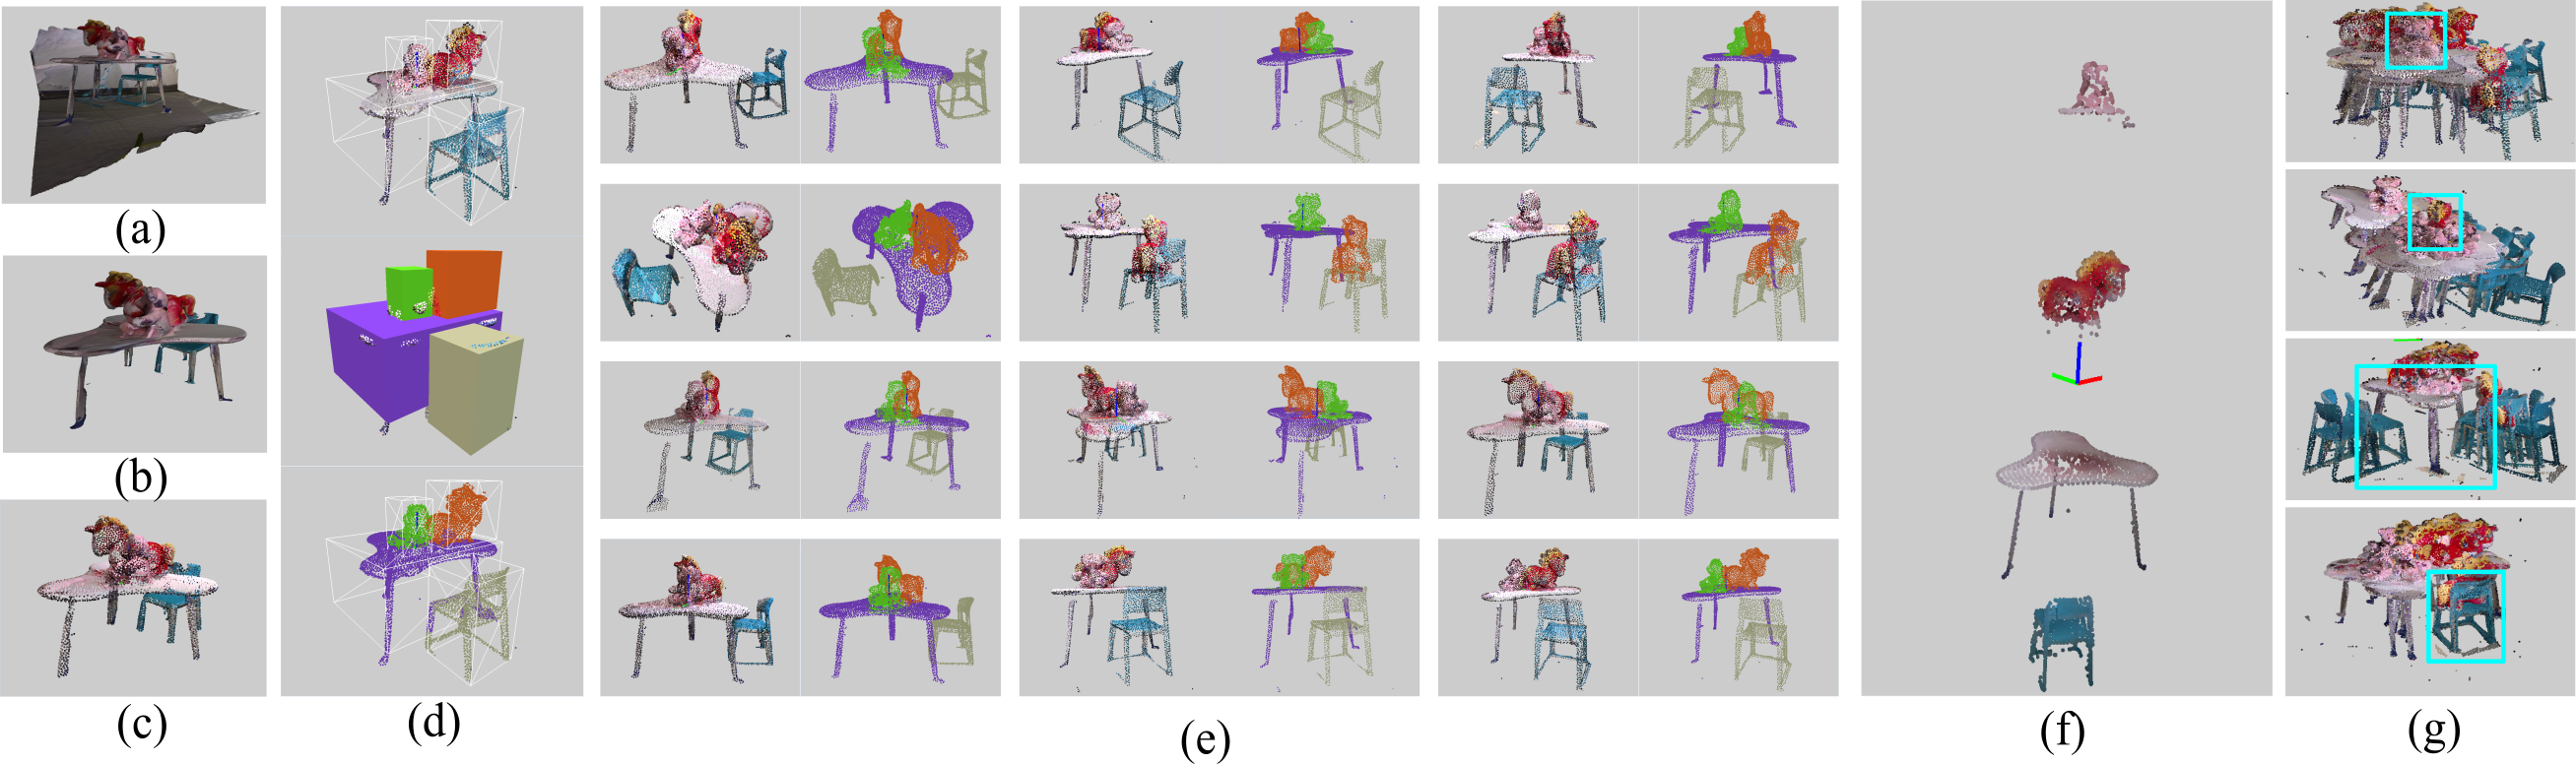
\includegraphics[width=\linewidth]{images/realdata/realdata}
	\caption{\label{fig:realdata}This figure shows our test on a real data. (a) shows how we capture real data with method in \cite{VXH} (b) shows result after we remove walls and floors by plane fitting (c) shows we generate point set with method in \cite{PossionSampling}. (d) shows the first input point set, the input layout on it and its segmentation result. (e) shows all other pairs of input point sets and corresponding segmentation result. (f) shows the final Gaussian centroids from top to down correpondent to different objects (g) verifys the registration result by aligning input point sets respecting to each object. The light blue rectangle highlights the object that is aligned together. }
\end{figure*}
To capture real data we employ the method of \cite{VXH} and use plane fitting to remove walls and floors. We then transfer the mesh into point set with the sampling process from \cite{PossionSampling}.
We test our algorithm on the sampled point sets. Figure~{\ref{fig:realdata}} shows the complete result of our test. On real data, there are noised color, shape distortion, partial scanning and outliers as they are highlighted in Figure~\ref{fig:challenge}. 
\begin{figure}
	\centering
	\includegraphics[width=\linewidth]{images/challenge/challenge}
	\caption{\label{fig:challenge}This figure highlights the common challenges on real data.}
\end{figure}
From Figure~\ref{fig:realdata}(e), we can see that all input point sets are partitioned into objects. From the Figure~\ref{fig:realdata}(g), we can verifys that the object from each input set are aligned together by the result transformation.  
\subsection{Limitations and Future Work}
The biggest problem holding us back is the time performance of current implementation of our tool.  Due to i.i.d. assumption most calculation of our algorithm can actually be parallelized. We plan to implement a new version on GPU cluster so that we can explore more potentials of our algorithm, for example,Try to integrate semantic feature vectors (generated by neural networks) into it and try it on a scene of larger scale like \cite{GOGMA}. As advocated in the recent work of \cite{AGM}, it may be a good idea to do the joint registration and co-segmentation with hierarchical GMM representation when applyed to scenes on a larger scale. 